% This is samplepaper.tex, a sample chapter demonstrating the
% LLNCS macro package for Springer Computer Science proceedings;
% Version 2.20 of 2017/10/04
%
\documentclass[runningheads]{llncs}
%
\usepackage{graphicx}
\usepackage{amssymb}
\usepackage{algorithmicx}
\usepackage{algorithm2e}
\usepackage[utf8]{inputenc}
\usepackage{subfig}
\usepackage{placeins}
% Used for displaying a sample figure. If possible, figure files should
% be included in EPS format.
%
% If you use the hyperref package, please uncomment the following line
% to display URLs in blue roman font according to Springer's eBook style:
% \renewcommand\UrlFont{\color{blue}\rmfamily}

\begin{document}
%
\title{Interactive Visualization of Large Bipartite Networks Assisted by Multilevel Strategies}
%\thanks{Supported by FAPESP, project 2017/05838-3}}
%
\titlerunning{Multilevel Visualization of Bipartite Networks}
% If the paper title is too long for the running head, you can set
% an abbreviated paper title here
%
\author{Renato Fabbri\orcidID{0000-0002-9699-629X} \and
Alan Valejo\orcidID{0000-0002-9046-9499} \and Alneu A. Lopes\orcidID{0000-0003-3112-4746}
Maria Cristina F. Oliveira\orcidID{0000-0002-4729-5104}}
%
\authorrunning{R. Fabbri et al.}
% First names are abbreviated in the running head.
% If there are more than two authors, 'et al.' is used.
%
\institute{University of São Paulo, São Carlos SP, BR\\
\email{renato.fabbri@gmail.com},
\email{alanvalejo@gmail.com},
\email{alneu@icmc.usp.br}
\email{cristina@icmc.usp.br}}
%\url{http://conteudo.icmc.usp.br/pessoas/cristina/}}
%
\maketitle
%
\begin{abstract}
% The abstract should briefly summarize the contents of the paper in
% 150--250 words.
  Bipartite, or two-layer, networks are pervasive
  in modeling real-world phenomena and play a fundamental role in
  graph theory.
  Multilevel methods, introduced for solving optimization problems on networks, have been applied to the problem of drawing simple (``unipartite'') networks, but not for interactive visualization of bipartite networks.
  In this work, we present a proof-of-concept implementation on the use of the multilevel method for this purpose. We developed a web-based visualization interface in which multilevel coarsening algorithms are applied to obtain a hierarchy of gradually simplified representations of an input  bipartite network.
  Node-link representations of the resulting network hierarchy can be presented to users following a genuine route of the ``overview first, zoom and filter, details on demand'' visual information seeking mantra, as analysts may depart from a coarser representation and select super-nodes or sub-graphs (network partitions) to be expanded and shown at greater detail. 
    Such a solution allows for interactive and intuitive navigation of large-scale network structures and can provide the basis for more elaborate visual mappings of network data sets. 
   
  
  %The application allows not only the visualization of large networks, but also for an on-demand navigation of the multilevel structure,  and is useful for the further development multilevel strategies themselves e.g. by the specification of vertices to guide the coarsening processes and  the examination of the resulting multilevel hierarchy.

\keywords{Network visualization \and Bipartite networks \and Multilevel strategies \and Big data \and Complex networks \and Data visualization}
\end{abstract}
%
\section{Introduction}
The visualization of large-scale networks poses challenges in terms of both the computational cost and the effective presentation of information~\cite{tang,staudt}.
These issues may be aggravated in the case of bipartite networks,
due to their sparsity and topological complexity.
In bipartite networks the set of nodes is split into two partitions called ``layers''
and links are not allowed between nodes in the same partition.
Such networks arise often and naturally from the representation
of relations between entities of two kinds,
e.g. documents and terms, papers and authors~\cite{doc,sci,movie}, or patients and genes~\cite{gene}.
Furthermore, real-world networks are often bipartite and most unipartite networks are actually projections of bipartite networks or exhibit bipartite properties~\cite{guillaume0,guillaume}.
%Multilevel strategies can be employed to assist the visualization and navigation of large networks, which consist on obtaining an incremental coarsening of the original network to yield a sequence of gradually simplified representations, i.e. with fewer nodes and links.

Multilevel strategies (see Section~\ref{des}) perform an incremental coarsening of an original
network to yield a sequence of gradually simplified representations, i.e. with fewer nodes and links.
They have been traditionally employed to enable executing expensive algorithms
on large-scale networks\footnote{By large-scale we mean networks with up to a few hundreds of thousands vertices, in contrast to massive-scale networks with  millions to billions vertices.}: the rationale is to run the algorithm on a coarsened
version that preserves the major properties of the input network to compute an initial solution, which is projected into the inverse hierarchy of coarsened networks  to yield a solution to the problem relative to the original network~\cite{alan2,ml2}. 
The method has been mostly applied to identify community structures in large networks~\cite{Pope2017}, but also to other problems, including computing node-link layouts of simple (i.e. ``unipartite'') networks~\cite{u1,u2,u3,u4,u5,u6,u7,u8,u9,u10}. We are aware of a single (yet unpublished) contribution in the context of bipartite networks, in which a visual metaphor is used to assist users executing multilevel methods~\cite{cintra2019}. In general, solutions for node-link visualizations of large networks often rely on aggregation of nodes in clusters or communities to reduce visual clutter and create simpler representations amenable to user interaction~\cite{a1,a2,a3,a4,a5,a6}. 

In this paper we present a system that employs the multilevel method to enable interactive visualization of large bipartite networks with node-link representations. Its underlying rationale is to present first a coarser instance of the network with which a user can interact to request for super-nodes (or groups of them) to be uncoarsened and visualized in more detail.
The resulting interface enables interactive navigation on large networks, e.g. by gradual and on-demand uncoarsening of super-nodes, combined with functionalities for zooming and requesting complementary information on nodes and links. Besides assisting in the analysis of data represented as bipartite networks, the visualization may assist developers of multilevel algorithms, e.g., for inspecting and comparing results yielded by different algorithm and parameter choices. 
%Visual analytics is the field dedicated to the science of analytical reasoning assisted by interactive visual interfaces~\cite{visAn}. It is specially concerned with coupling interactive visual representations to support sense and decision making. The visual analytics techniques are most often employed to amplify human capabilities in specific ways, which includes reducing the search space, enhancing the recognition of patterns and the inference of relationships, and providing a manipulable medium for exploring and identifying the information of interest.
%For this solution to be properly characterized as a visual analytics contribution, the methods and software described in Sections~\ref{des} and~\ref{sof} should further enable the discovery of information, such as metadata associated with  network nodes and links (e.g. authors, words or documents).
%Accordingly, our methods and software may be understood as data visualization with explicit visual analytics elements, such as interactivity, on-demand supply of information, and selective navigation.
We consider the current implementation as a proof-of-concept to demonstrate the feasibility of using the multilevel method to support effective visualization of large bipartite networks using node-link views.
%Most importantly, the overall method, and the implemented interface, is a proof-of-concept, it demonstrates the feasibility of the use of multilevel strategies for the efficient visualization of large bipartite networks.

%This paper is organized as follows. 
%in Section~\ref{rel} the related work is examined, while in~\ref{nom} are selected remarks about the vocabulary.
%The method is delineated in Section~\ref{des} and the software implementation is described in Section~\ref{sof}.
% Results and discussion are in~\ref{res}. Finally, Section~\ref{con} holds conclusions and further work envisioned.

%\subsection{Related work}\label{rel}
%%%
% incrementar? no artigo do alan tem mais informação sistematizada
% citar mais trabalhos desenvolvidos no ICMC?
% tratar mais especificamente de visualização de redes bipartidas?
% tratar mais especificamente de estratégias multinivel?
%Multilevel strategies have been employed to visualize unipartite networks~\cite{u1,u2,u3,u4,u5,u6,u7}.
%Also, the aggregation of clusters has been reported, an approach that resembles a coarsening procedure in creating simplified representations of an input network~\cite{a1,a2,a3,a4,a5,a6}.
%We are not aware of previous reports on the use of multilevel strategies for the visualization and navigation of bipartite networks.
%Furthermore, few contributions~\cite{a1,a2,a3,a4,a6} report on interactive systems for network visualization, and these do not tackle the usage of multilevel strategies for this purpose.

%\subsection{Remarks on nomenclature}\label{nom}
%%%
% remover seção?
% multiplex, ?
% multilevel strategies synonym for optimization algorithms?
%The main vocabulary issue that arises in the context of this article is between level and layer. Layers are the (two) node partitions of a bipartite network, while levels comprise the sequence of coarsened networks.
%Also, simple or homogeneous networks are opposed to heterogeneous networks, in which there are more then one type of node.
%Bipartite networks may be regarded as an elementary case of heterogeneous networks, but it has one additional restriction: only nodes of different types are connected.
%Another usual concept in this context is that of a multilayer network, in which there are layers, i.e. partitions of nodes, in addition to nodes and links.
%Bipartite networks, in this case, are multilayer networks with only two layers and no intra-layer links, i.e. all the links are inter-layer.
%Most importantly, there are many synonyms which are found in this context, e.g. supernodes are also called metanodes or supervertices.
%A thorough exposition of the vocabulary is beyond the scope of this article, but some attention for the issue is helpful to assist searches and newcomers.

\section{A brief description of the multilevel method}\label{des}

In this section we address two topics. First we introduce some fundamental concepts and present an overview of the multilevel method in the context of bipartite networks. Then we outline how it can be instantiated to support interactive navigation  on such networks. 

%\subsection{Fundamental concepts}
\subsection{Multilevel coarsening of bipartite networks}\label{smul}
A bipartite network $G=(V,E)$ consists in a set $V$ of nodes which is partitioned in two subsets
with no links between nodes in the same set, i.e. $\exists\; V_1, V_2:\; V_1\cup V_2 = V,\;V_1\cap V_2 = \emptyset$, and $E\subseteq V_1 \times V_2$.
The variable names are borrowed from traditional
graph (network) theory, with Vertices (nodes) and Edges (links).
One may regard the network as $G=(V,E,\sigma,\omega)$, with
$\sigma\,:\,V\rightarrow \mathbb{R}^*$ and $\omega\,:\,E \rightarrow \mathbb{R}^*$,
where $\sigma(v)$ is the weight of the node $v$ and
$\omega(u,v)$ is the weight of the link $(u,v)$.

%The multilevel optimization method is a meta-heuristics employed to guide, modify and potentially fix a solution obtained from a target algorithm. 
%In the context of network problems, the method creates a hierarchy of coarsened networks $G_l$, $l$ integer $ \in [0,L]$ where $G_0$ is the original network and $|V_i| \geq |V_{i+1}|$. It operates in three phases, as illustrated in Figure~\ref{mlf}: coarsening, solution finding and uncoarsening, where a solution found in the coarsest network instance $G_L$ is projected back to the original, uncoarsened, network $G_0$.

%The coarsening procedure requires two algorithms, the \emph{matching}, which defines the nodes to be collapsed, and the \emph{contraction}, which builds the reduced representation from the matched nodes.
%Several coarsening algorithms have been reported in the literature~\cite{co1,co2}, a detailed exposition is beyond the scope of this paper. 

%and a few have been recently introduced for bipartite networks~\cite{alan2}.

%, it has been shown that existing coarsening algorithms for bipartite networks can yield simplified models that preserve the essential topological features of the original networks~\cite{alan2}, as discussed further in Section~\ref{sof}.

%Visual analytics is the scientific field dedicated to analytical reasoning assisted by interactive visual interfaces~\cite{visAn}. Therefore, the area is specially concerned with coupling interactive visual representations with sense and decision making. Of special relevance for the present work, the techniques are most often employed to amplify human capabilities in specific ways, which includes reducing the search space, enhancing the recognition of patterns and the inference of relationships, and providing a manipulable medium for the exploration of the information of interest.
%For this present work to be better characterized as a visual analytics contribution, the methods described in this section and software described in Section~\ref{sof} should further enable the discovery of information, such as metadata of the networks (e.g. authors, words or documents).
%Accordingly, our methods and software may be understood as data visualization with explicit visual analytics elements, such as interactivity, on-demand supply of information, and selective navigation.


%\subsection{Multilevel coarsening of bipartite networks}
The multilevel optimization method is a meta-heuristics employed to guide, modify and potentially fix a solution obtained from a target algorithm. 
It operates in three phases, as illustrated in Figure~\ref{mlf}, namely coarsening, solution finding and uncoarsening.
Valejo et al.~\cite{alan2} introduced a general framework applicable to bipartite networks. They presented novel and efficient matching and coarsening algorithms and validated them in problems of community detection and dimensionality reduction. They also provided empirical evidence that the proposed coarsening algorithms preserve the essential topological features of an original input bipartite network. Here we delineate the stages of the multilevel method in the context of our bipartite network visualization contribution.

%The multilevel optimization method is a metaheuristics employed to guide, modify and potentially fix a solution obtained from a target algorithm.
%It is split into three phases, as illustrated in Figure~\ref{mlf}: coarsening, solution finding and uncoarsening, where a solution found in the coarsest network instance $G_L$ is projected back to the original, uncoarsened, network $G_0$.

%Figure~\ref{mlf} illustrates such process.

\begin{figure}\centering
 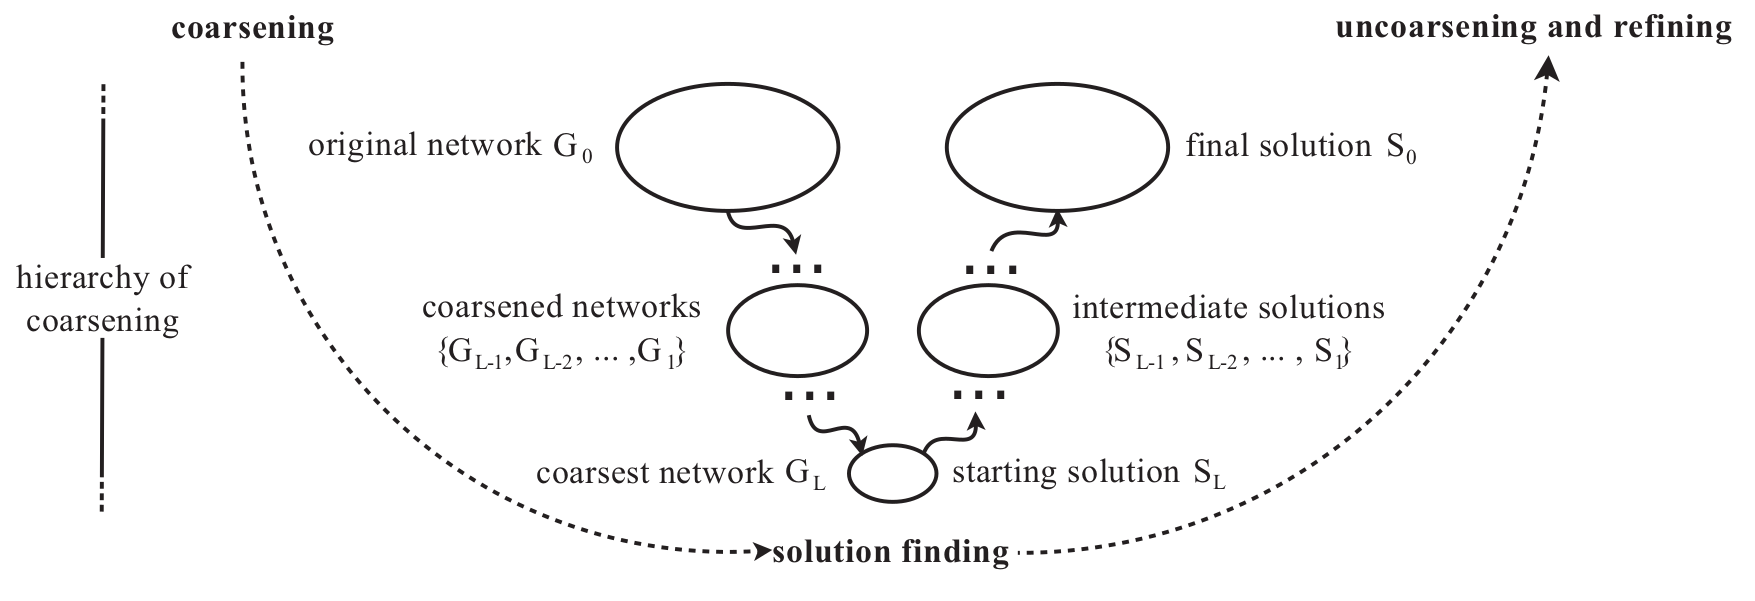
\includegraphics[width=\textwidth]{mlf}
  \caption{Phases of the general multilevel optimization method.
  A sequence of incrementally reduced networks is obtained in the coarsening phase.
  An initial solution is found applying a target algorithm in the coarsest network instance in the solution finding phase. This solution is projected back to the initial, uncoarsened, network in the uncoarsening phase.
  %Further details are given in Section~\ref{des} and specificities related to these phases when applied to interactive data visualization are in Sections~\ref{net} and~\ref{nav}.
  }\label{mlf}
\end{figure}

The coarsening phase creates a hierarchy of coarsened networks $G_l$, $l$ integer $ \in [0,L]$ where $G_0$ is the original network and $|V_i| \geq |V_{i+1}|$, resulting in a hierarchical representation of $G_0$ at decreasing levels of detail.
The process is carried out by two algorithms: \emph{matching}, which decides which nodes to merge,
and \emph{contracting}, which computes a reduced representation from the input network and the matching.
In general, pairs of nodes are selected to be merged into super-nodes, and
most often a matching $M$ consists of a set of non-adjacent links,
i.e. $\forall\; l_1, l_2 \in M, u \in l_1 \Rightarrow u \notin l_2$~\cite{co1,co2}.
%The heavy-edge matching, for instance, fits this canonical description attempting to maximize total matching weight, but the matching may not satisfy such restrictions.
%Matching strategies based on selecting cliques or other larger node sets to be merged into super-nodes are possibilities under development.
%%%
% citar alguem aqui?
For bipartite networks, we rely on the matching algorithms introduced by Valejo et al.~\cite{alan2} in which the matching must satisfy two restrictions:

\begin{itemize}
  \item A node may only match nodes on the same layer.
  \item A node may only match nodes that are reachable in two hops, i.e., via paths formed by two successive links    (i.e.  the closest possible nodes in the same layer).
\end{itemize}

The matching is followed by the contraction of the network into a coarser form.
Typically, the nodes matched are merged into a super-node weighted according to the number of of its composing nodes, and the links incident to such nodes are joined into super-links,
weighted based on the accumulated weights of the links merged.
The solution finding phase usually involves executing a computationally expensive algorithm, which becomes feasible in the coarsest network. In the uncoarsening phase the solution found in the coarsest network instance $G_L$ is projected back to the original, uncoarsened, network $G_0$. Uncoarsening is thus performed across the complete hierarchy, from $G_L$ to $G_0$ with successive refinement of the solutions to avoid local minima and improve solution quality.
%These two phases are substantially different when the multilevel strategy is applied to visualization, which motivated their separate exposition in the next subsection.

%\subsection{Network visualization assisted by multilevel strategies}\label{net}
In applying the general multilevel framework to obtain an interactive visualization solution, some adaptations are in order.  
%Such adaptations for our interactive visualization solution is as follows.
In this scenario the goal is to obtain a visual mapping of the network, i.e. the solution finding phase corresponds to computing a layout of $G_L$ suitable for presentation.  Uncoarsening is performed  on-demand, through specific user requests
to expand selected network super-nodes for more detailed visualization, which is possible displaying them at the subsequent hierarchical level. The procedure is delineated in the BiNetVis algorithm (Algorithm~\ref{alg}) and further detailed in Sections~\ref{nav} and~\ref{sof}.

This solution avoids unnecessary complexity and, most importantly, avoids overloading the visualization with information beyond the cognitive convenience of the user and the computational power available to ensure real-time interactivity.
Users can interact to specify the desired coarsening algorithm, select the node-link drawing algorithm, select the target super-nodes for uncoarsening, navigate the network, access data and metadata, tune the visual mapping options, for instance to modify colors and resize and move nodes. 
%Interactivity is crucial for a number of reasons: the specification of the coarsening algorithm; the definition of the uncoarsening desired; to enable the navigation of the network, including the access to metadata and changes to the visualization achieved; and for tuning the achieved visual mapping status, such as by resizing and moving nodes.
%The procedure is delineated in Algorithm~\ref{alg} and further detailed in Sections~\ref{nav} and~\ref{sof}.


\SetKwData{Matching}{Matching$_b$}
\SetKwData{Contracting}{Contracting$_b$}
\SetKwData{map}{map\_to\_screen}
\SetKwData{trans}{transform\_visual\_mapping}
\SetKwInOut{Return}{Return}
\begin{algorithm}
  \qquad\qquad\qquad{\bf\emph{BiNetVis Algorithm}}\\
  \vspace{0.3cm}
  \KwIn{\\
  \quad bipartite network: $G$\\
  \quad maximum number of levels: $L \in [0,n] \subset \mathbb{Z}$\\
  \quad reduction factor for each layer: $rf_1, rf_2 \in (0,0.5] \subset \mathbb{R}$.\\
  \quad layers to be coarsened: $layers \in \{1,2\}$\\
  \quad user command given through the visual interface: $C$
  }
  \KwOut{\\
  \quad Visual mapping of the network: $V$}
  \BlankLine
  $i \leftarrow 1$\;
  \While{$i \le$ layers}{
    $l\leftarrow 1$\;
    \While{$l\leq L$}{
      $M \leftarrow$ \Matching{$G_l$, $i$, $rf_1$, $rf_2$}\;
      $G_{l+1} \leftarrow$ \Contracting{$G_l$, $M$}\;
      increment $l$\;
    }
      increment $i$\;
  }
  $V \leftarrow$ \map{$G_L$}\;
  \While{$C$ is not '$exit$'}{
    $C\leftarrow$ user command\;
    $V\leftarrow$ \trans{$V$, $C$}\;
  }
  \caption{
An algorithmic description of the multilevel method adapted for the visualization of bipartite networks, named the {\bf \emph{BiNetVis Algorithm}}.
  The routines {\bf Matching$_b$} and {\bf Contracting$_b$} refer to any matching or contracting
  algorithms applicable to bipartite networks~\cite{alan2}.
  The routine {\bf map\_to\_screen} may refer to any node-link layout algorithm followed by a rendering of the network to the screen.
  The user may then modify the visual mapping, e.g., request to uncoarsen selected super-nodes or use any of the other interaction commands available,
  such as request metadata, change node position, change node and link color or transparency, perform zoom and pan, etc., as described in Section~\ref{sof}.}\label{alg}
\end{algorithm}

\subsection{The navigation pathway}\label{nav}
The abundance of information within large-scale networks makes pertinent the
application of the well-known ``visual information-seeking mantra''~\cite{shneiderman1996eyes}:
\emph{overview first, zoom and filter, then details-on-demand}.
This mantra embeds a number of visual design guidelines,
such as the details-on-demand interaction strategy, and provides
a widely acknowledged framework for designing information visualization applications. The navigation pathway supported by the current implementation of the proposed solution is illustrated in Figure~\ref{fnav}.
Accordingly, exploration starts with an overview yielded by the visual mapping of the coarsest network instance, obtained using standard layout algorithms for node-link diagrams.
The user may then zoom into specific network regions and request
details using several operations, most importantly:
\begin{itemize}
  \item Reposition nodes, expose linking patterns.
  \item Request metadata, e.g. for a node one may ask for its degree, or how many predecessors it has in the previous level, or how many successors in the subsequent level.
  \item Adjust the visual mapping of network features, such as map the size of glyphs representing nodes to node degree or to the number of node predecessors, or modify link transparency.
  \item Request the uncoarsening (i.e., expansion to the upper level) of a selected super-node or group of super-nodes.
\end{itemize}

Other operations are convenient to adequate the visual mapping to the current user needs, e.g., setting the network size, expanding super-nodes, exposing levels and highlighting topological features. These operations are further detailed in Section~\ref{sof}.


\begin{figure}\centering
 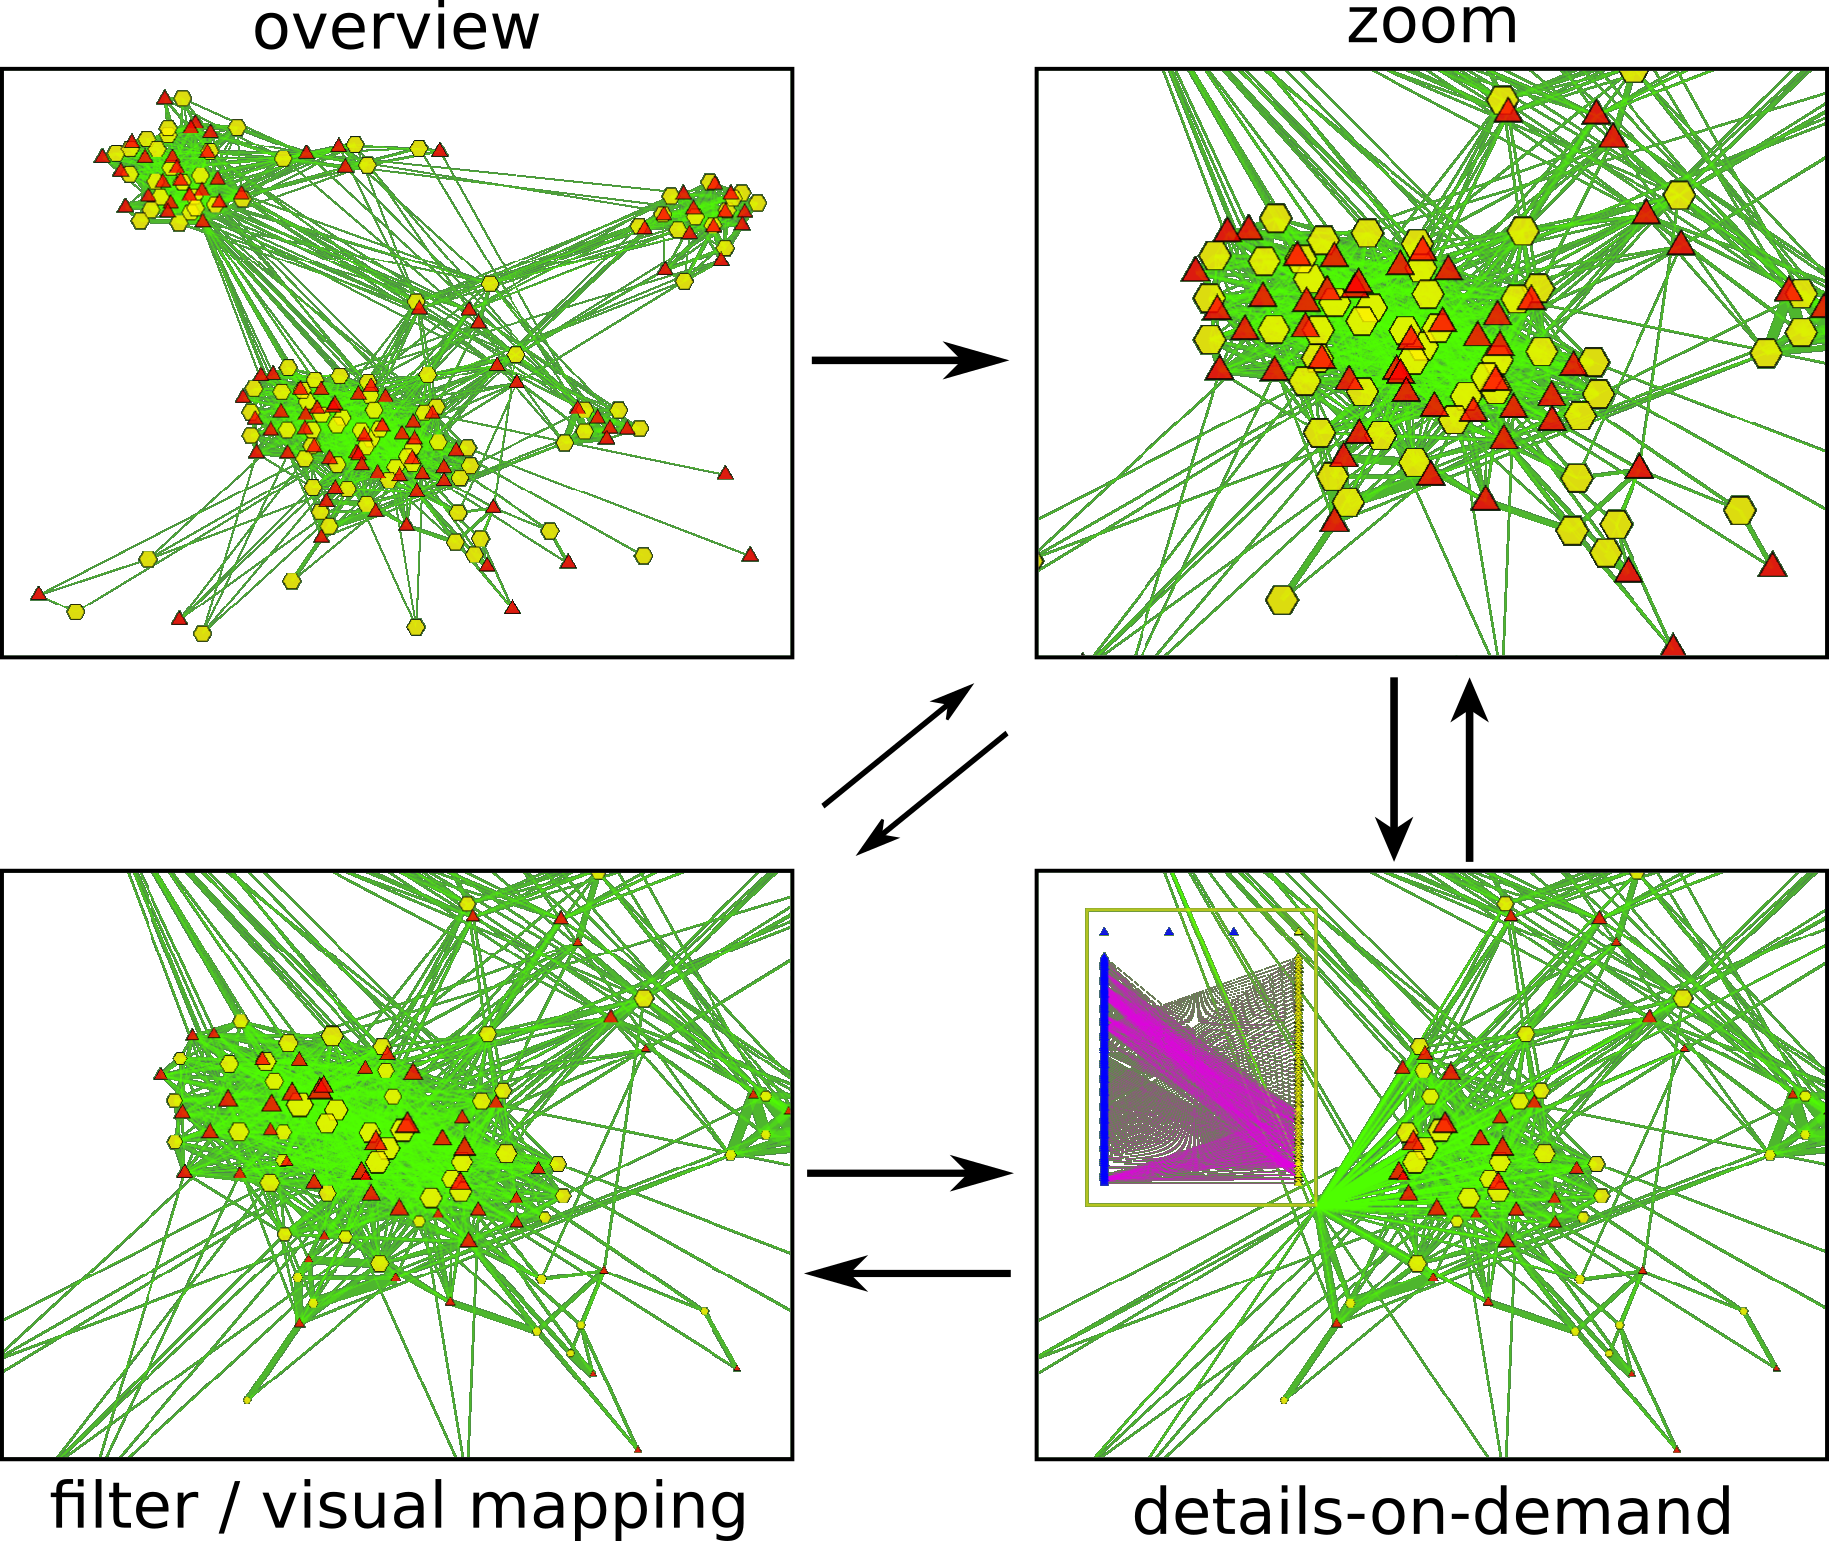
\includegraphics[width=0.7\textwidth]{fnav____}
  \caption{The navigation pathway on bipartite networks made possible using the multilevel method coupled with auxiliary interaction tools.
  Compliant with the ``visual information seeking mantra''~\cite{shneiderman1996eyes}, initially it displays a view of the bipartite network in its coarsest form.
  The user may then zoom-in into regions and select specific nodes or all nodes within a region to inspect and visualize in further detail, apply filters and modify the visual mappings of topological elements, or request to see the corresponding nodes in further detail, drilling-down to the next network level.
  These operations are user-driven and may be carried out in any sequence.
  }\label{fnav}
\end{figure}

\noindent 
\section{Software implementation}\label{sof}
% optimization of the computational capacity for large networks by
% means of Web GL, triangles for nodes and details on demand
We implemented the framework described in Section~\ref{des} using scientific,
database and web resources, making it available within a web page
for use through simple mouse-driven actions and requiring no software installation beyond a web browser. % such as Firefox or Google Chrome.
The software has been named BiNetVis (from Multilevel Bipartite Network Visualization)
and is exemplified in Figures~\ref{fpage0},~\ref{initial} and~\ref{secondPhase}.
In the following we describe its functionalities and the underlying technologies.

\begin{figure}\centering
 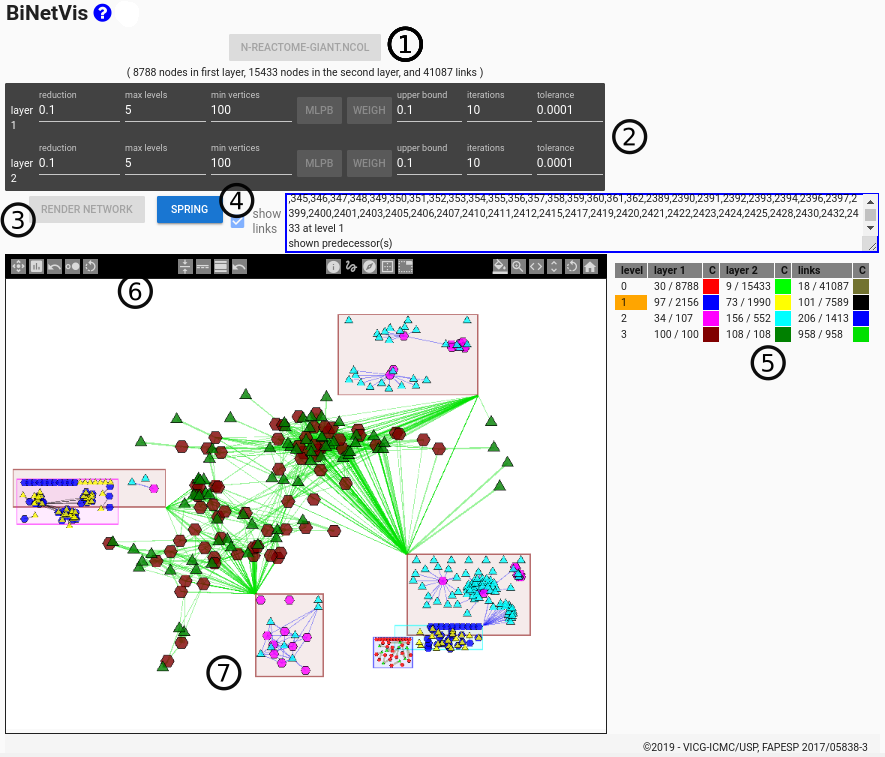
\includegraphics[width=\textwidth]{overall2_}
  \caption{The BiNetVis interface: (1) drop-down menu for selecting or uploading a network for analysis;
  (2) control widgets to select and parameterize the coarsening algorithm;  (3) the render button to display the network; (4) auxiliary widgets for selecting the network layout, show/hide links, and area to display user requested information on nodes or links; (5) interactive table holding information about the multilevel hierarchy levels and the bipartite network layers; can also be used to set the visualization on the canvas; (6) toolbar with controls for navigation of the network and fine-tuning the visualizationi, better inspected in Figure~\ref{toolbar} of Appendix C; (7) canvas with the node-link representation of the multilevel network. Notice that nodes shown belong to four distinct hierarchical levels: level 3 (dark red/green), level 2 (pink/cyan), level 3 (navy blue/yellow) and level 2 (red/bright green). The current interaction focus in on level 2, as indicated by the orange mark. 
 %Elements are described in further detail in Section~\ref{use}.
  }\label{fpage0}
\end{figure}

\subsection{Using BiNetVis}\label{use}
% network upload, format.
% layouts available
% algorithms available for coarsening, and their parametrization
% initialization of the visualization: click on render
% tools available and their operation
In using BiNetVis, the analyst first uses a drop-down menu to select a network of interest, s/he may also upload a new network using the same menu. The next step is to select one of the available network layout algorithms and possibly tune the coarsening algorithm, as illustrated in Figure~\ref{initial}, although default settings are reasonable for a newcomer.
Once the ``render network'' button is hit the network node-link representation is mapped to the screen according to the selected layout algorithm.
Subsequent usage relies on manipulation of the visual mapping controls presented on the
canvas by means of user actions and related mouse operations.
These steps are illustrated in Figure~\ref{fpage0}.

\begin{figure}\centering
 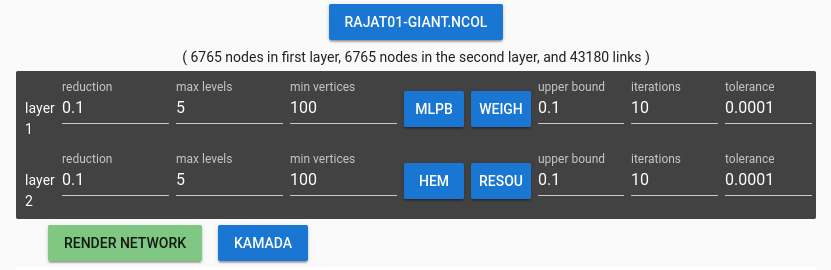
\includegraphics[width=\textwidth]{initial_}
  \caption{The initial step of the BiNetVis usage is to apply the multilevel coarsening to an input network.
  The button at the top is for network uploading and selection.
  In the gray box, the user chooses the coarsening algorithm and sets its parameters, as detailed in the Appendix A. % Appendix~\ref{ap}.
  The blue button at the bottom is a drop-down menu where the user can select the node-link layout algorithm, where multiple alternatives are provided.
  The green button renders the network to the canvas and initializes further control widgets.
  By hitting the green button, except for the layout  button all the control elements above are disabled as the interface enters the visualization mode.
  %Further information is given in Section~\ref{use}.
  }\label{initial}
\end{figure}

The multilevel method yields a hierarchical representation of the network at decreasing levels of detail (as depicted in Figure~\ref{mlf}), where the number of hierarchy levels is an input parameter to the coarsening algorithm. The proposed visualization initially shows a node-link representation of the the coarsest network $G_L$ (the upper level instance) showing it at the minimum level of detail. The network $G_L$ is thus the initial focus of user interaction. The focus can be directed to other levels of the multilevel hierarchy, but a single level can be the current focus to which any interaction actions will apply.
%to the representation at the level defined as the current focus.
%There are multiple levels of representation entailed by the multilevel strategy.
%This makes pertinent that one and only of the available levels is explicitly selected so that the transformations are performed on that level.
Thus, there is always a user-selected level to which interface controls apply, such as link coloring or expanding super-nodes to reveal their predecessor nodes.
As the reader may infer, the numbers of visible nodes and links in each level are not fixed throughout the navigation.
The user can modify the focus level in the table to the right of the canvas, as shown in Figure~\ref{secondPhase}, which also shows the number of visible and total nodes and links at each level.
The user may also interact with the table to modify node color and shape or link color at any layer/level, as well as toggle show/hide links with left/right clicks on the corresponding colored cell.

\begin{figure}\centering
 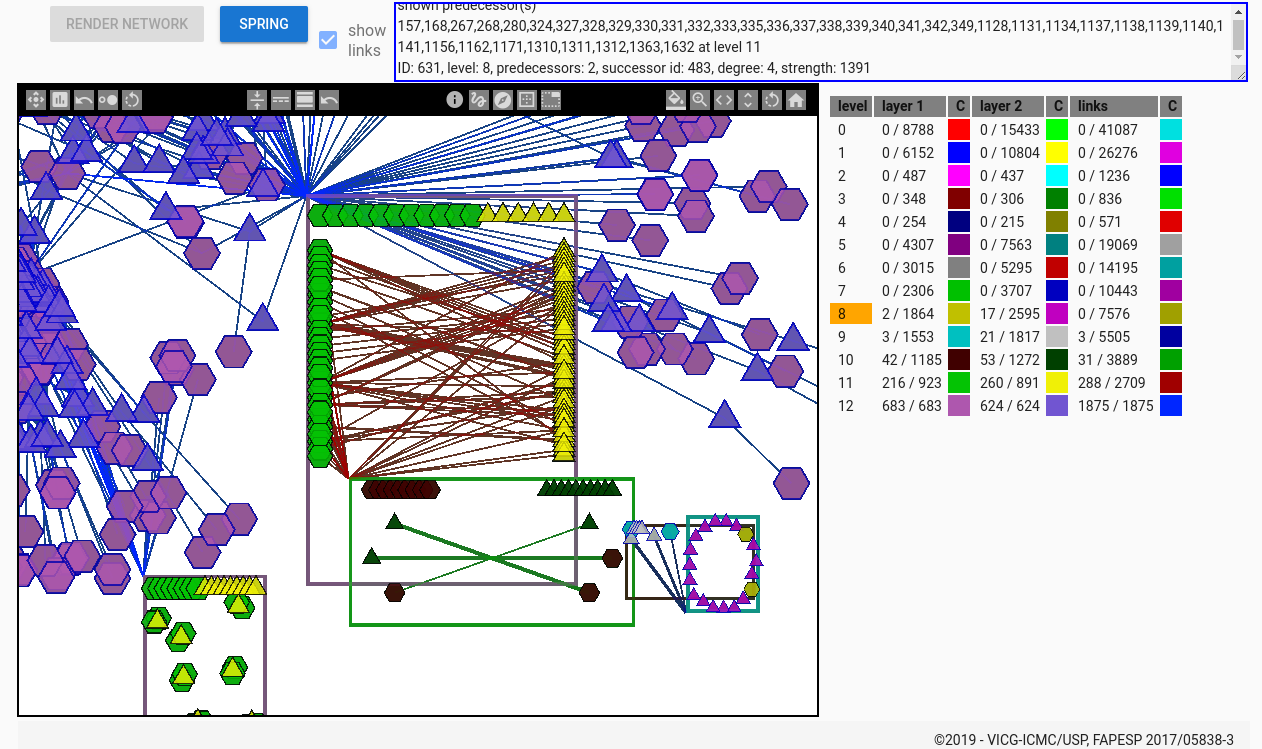
\includegraphics[width=\textwidth]{secondPhase_}
  \caption{Interface elements in BiNetVis in the visualization mode, where the user can navigate in the network and modify visualization settings.
  S/he may change the layout used when super-nodes are expanded and their predecessors rendered.  The checkbox to the left of each level may be used to show or hide the corresponding links at the level.
  The text area displays user-requested information or information useful for navigation.
  The canvas holds the node-link representation of the network, possibly depicting nodes at multiple levels of the multilevel hierarchy. The node-link representation may be modified using the toolbar controls and the controls the table on the right, which also shows key information on the status of the visualization. Here the current focus is on level 8 from a multilevel network with 12 hierarchical levels. 
  %Further information is given in Section~\ref{use}.
  }\label{secondPhase}
\end{figure}

The toolbar on top of the canvas in Figure~\ref{secondPhase} holds further controls organized in groups according to their target interface element.
The first group of controls affect graphical attributes of nodes: size mapped to degree or to number of predecessors, reset size, modify transparency and rotation.
The second group affects link properties: thickness, transparency, proportionality to weight
using thickness or transparency, and reset proportionality.

The third group refers to controls more specific to how BiNetVis operates as a multilevel visualization. 
%are selected to make mouse operations entail special processes and transformations of the visualization.
The first control returns information relative to a selected (clicked) node:
id, level, number of predecessors at the upper level, successor id (if applicable), degree, strength (sum of link weights).
%Other information the analysts report necessity of are easily implemented, but currently only these items are returned to avoid unnecessarily flooding the text area.
The second control allows moving nodes: specific nodes are moved if clicked and dragged; a rectangular region can be defined (clicking on an empty region in the canvas and dragging then releasing the mouse) to move all nodes within. The third control allows expanding super-nodes to expose their predecessor nodes and links. Again, the user specifies a rectangular region and the super-nodes within are bounded within the region and replaced with their predecessor nodes, which exist at the upper hierarchical level (thus at a greater level of detail). Thus, an expanded super-node is identified by a bounding rectangle that contains a view of its predecessor nodes and links.
%are drawn inside this region.
The same control can be employed to join expanded super-nodes, but it was found convenient to include a fourth control to assist in this task, which allows joining two expanded super-nodes by clicking on them in sequence.
The final control in this group supports three operations on expanded super-nodes:
if an expanded super-node is clicked on and dragged its rectangular shape is resized accordingly;
if the super-node is clicked on and released (no dragging) its links  to the other super-nodes are shown attached to the next counterclockwise corner of the bounding rectangle.
When the expanded super-node is resized the spatial layout of its child nodes is optimized to the modified drawing area. This is most useful in combination with the drag tool, to rearrange the nodes at the finer level of detail in a more compact disposition.
Upon a super-node resize the child nodes are rearranged to fit the new rectangular area.
The final set of controls act on the canvas: they allow
changing the background color, zooming, left-right/up-down panning,
rotating the entire network, and toggling between the current zoom and pan configuration and the initial settings.
%The toolbar is contextualized in Figure~\ref{secondPhase}.

There are many subtleties on the orchestrated use of these controls.
As a facilitated means to convey the navigation possibilities, the user is invited to watch a demo video~\footnote{\url{http://rfabbri.vicg.icmc.usp.br:3000/multilevel2/about}} %in~\cite{yvideo}
and use the BiNetVis interface~\footnote{\url{http://rfabbri.vicg.icmc.usp.br:3000/multilevel2/topdown}}.
Furthermore, a simple case study is described in Appendix B.
%\cite{mbnvpage}.
The more seasoned software developers may browse the code, upload a local instance of the software, and make changes to its source code~\footnote{ https://github.com/ttm/netText}.
%\cite{mbnvcode}.

\subsection{Underlying software technologies}
% coarsening algorithms
% flask for server, feather for auxiliary server
% mongodb filesystem for data
% Nuxt/Vue.js for the frontend with heavy use of PIXI.js
Most important components of BiNetVis are written in a combination of JavaScript and Python: it uses Vue.js (set up by Nuxt.js) in the frontend client, the backend is a Flask Python server, used to perform specialized or heavy calculations.
A secondary server, a FeatherJS, is used to facilitate contact with the database and real-time multi-user interaction.
The data is stored in a MongoDB database and ordinarily in the file system,
while the multi-user interaction is deactivated for now to avoid unnecessary complexity.
Multiple coarsening algorithms for bipartite networks available from a previous implementation~\cite{alan2} are accessed by the Flask server.
The fast WebGL 2D rendering on the canvas is performed using Pixi.js.

%Scene rasterization is usually performed though triangles.
In order to comply with the goal of handling large bipartite networks, the network geometry on the canvas uses only triangles as primitives (for nodes) and straight lines (for links).
The user may wish to further alleviate the computational burden by not rendering the links.
To emphasize the bipartite nature of the network and render the visualization more aesthetically compelling the user may modify the node shapes in one (or both) layers to hexagons, instead of triangles.
Using these features, and within the technologies described, we have visualized networks
with tens of thousands of nodes without perceiving any lag in the interactive navigation and transformations,
with links shown,
even when running the system on ordinary machines, e.g. with 8GB RAM DDR3, a first generation i7 processor and a 1GB GPU.

%This is a brief account of the resources implemented in BiNetVis, the interested reader is welcome to browse the software code and documentation and contact the authors.
%~\cite{mbnvcode}.

% \section{Results and discussion}\label{res}
%%%
% consistent use of overview first, details on demand
% a first contribution on ML vis. of bipartite networks
% simple interactivity strategies
% enhancements of the navigation through the use of being-developed coarsening algorithms
% the use of the interface for guiding coarsening (through markers)
% the use of the interface to analyse coarsening results

% technologies used: maybe simpler if using meteor.js
% and simpler to achieve multiuser interactivity

\section{Conclusions and further work}\label{con}
%%%
% extension to multipartite (or heterogeneous) networks.
We introduced a visualization interface for bipartite networks
assisted by the multilevel method that admits a conceptual organization very consistent with the well-known visual information seeking mantra stated as \emph{overview first, zoom and filter, then details-on-demand}. As exemplified in the software description, it allows users to obtain an overview of the major topological structures in a network and then focus on relevant elements for which further details can be displayed.
The combination of the multilevel strategy with suitable software technologies and computationally inexpensive design decisions regarding
the rendering of node-link representations yields a visual interface manageable with simple interactive operations that can effectively display large-scale networks. In summary, this software is introduced as a proof-of-concept on the feasibility of employing multilevel strategies for using the familiar node-link views  to visualize large bipartite networks. The same underlying rationale is applicable to unipartite and to heterogeneous networks as long as the underlying multilevel methods are provided.

The proposed visualization solution could be incorporated into a visual analytics environment for large networked datasets, with added tools to enable data analytics. It does require further validation on practical analytical settings, as the  usage scenarios of interactive knowledge discovery are inherently complex.
We believe that tuning this implementation into a tool to guide and inform developers of novel multilevel algorithms and applications would also be an interesting development. For instance, certain multilevel strategies require selecting pivot nodes to guide the coarsening procedure, a task that could benefit from an interactive visual interface. The same applies to developers who wish to compare the outcome of  multiple executions of coarsening algorithms, e.g., with different parameter settings.   


%In further steps, the navigation may be enhanced in multiple ways. 
%by the acute use of in-development coarsening algorithms.
%The system may be useful to assist the development of novel multilevel strategies, which should be verified. There are multilevel strategies that involve the selection of nodes as pivots to guide the coarsening procedure, a process to which there is no visual interface, and to which BiNetVis could be adapted.
%The interface is also envisioned to assist the analysis of coarsening results. In the current version of BiNetVis the analyst is able to scrutinize linking patterns and overall network structure though the node-link diagram, and request information, but it should be enhanced, e.g., to display histograms and global measures relative to each level.
%On the analysis of the networked structures, the navigation involving metadata, such as from genes and proteins, or from  documents and authors, should result in a visual analytics interface for interactive knowledge discovery.
%Finally, bipartite networks are naturally extended to heterogeneous (or multipartite) networks, and thus all the content of this article, and should require further research and development for the achievement of concrete derivatives.

\subsubsection*{Acknowledgements}
The authors acknowledge the financial support of the S\~ao Paulo State Research Foundation (FAPESP grant 2017/05838-3) and the National Council for Scientific and Technological Development (CNPq, grant 301847/2017-7).  The views expressed do not reflect the official policy or position of FAPESP or CNPq.

%\appendix

%\section{Choice and fine-tuning of the coarsening algorithm}\label{ap}
%The elements in Figure~\ref{initial}.

\bibliographystyle{splncs04}
\bibliography{biblio}
%
% \begin{thebibliography}{8}
% \bibitem{ref_article1}
% Author, F.: Article title. Journal \textbf{2}(5), 99--110 (2016)
% 
% \bibitem{ref_lncs1}
% Author, F., Author, S.: Title of a proceedings paper. In: Editor,
% F., Editor, S. (eds.) CONFERENCE 2016, LNCS, vol. 9999, pp. 1--13.
% Springer, Heidelberg (2016). \doi{10.10007/1234567890}
% 
% \bibitem{ref_book1}
% Author, F., Author, S., Author, T.: Book title. 2nd edn. Publisher,
% Location (1999)
% 
% \bibitem{ref_proc1}
% Author, A.-B.: Contribution title. In: 9th International Proceedings
% on Proceedings, pp. 1--2. Publisher, Location (2010)
% 
% \bibitem{ref_url1}
% LNCS Homepage, \url{http://www.springer.com/lncs}. Last accessed 4
% Oct 2017
% \end{thebibliography}

\appendix

\newpage
\section*{Appendix A: Coarsening parameters}

Table \ref{tab:parameters} lists the input parameters of the coarsening algorithms, which can be applied independently to one or to both network layers. 
%to fit their corresponding parameters. 
Three parameters are common to all algorithms, namely the maximum number of coarsening levels~\textit{max-levels}, a reduction factor~\textit{reduction} and a similarity function~\textit{similarity}, which returns a similarity score between a pair of vertices. Parameter ~\textit{reduction} is multiplied by the number of vertices to determine the maximum number of nodes matched, e.g. if $reduction = 0.5$ each coarsening iteration will (potentially) reduce the number of nodes by a factor of two, yielding a logarithmic decrease in network size along the process. 
%Similarity defines the distance between two vertices, in which a high similarity score represents a high degree of similarity. 
A possible similarity function is the \emph{common neighbors} metric, which returns the number of common neighbors between the two nodes. The default coarsening algorithm in the system is $MLPb$, which requires four additional parameters: \textit{min-vertices}, which is the minimum number nodes expected in the coarsest network and two parameters that serve as stopping criteria, namely a \textit{maximum number of iterations} and a \textit{tolerance} threshold. The algorithm stops if either the maximum number of iterations has been reached or the number of label updates is bellow the defined tolerance. 
A final parameter, namely \textit{upper bound}, defines an upper limit on the weights of super-nodes, which is useful to create super-nodes more faithful to the original structures and to avoid super-node weights that deviate significantly from the average values.
%that can be manipulated to create the coarsening networks.

\begin{table}[!ht]
    \centering
	\caption{Parameters of the multilevel coarsening algorithms (see Section~\ref{smul}). The rightmost column reports the default values. }
	%algorithms that use the respective parameter.}
	\label{tab:parameters}
 	\renewcommand{\arraystretch}{1.3}
 	\renewcommand{\tabcolsep}{0.45cm}
    \begin{tabular}{lrr}
    	\textbf{Parameter} & \textbf{Domain} & \textbf{Default} \\
    	\hline
    	%matching & string & MLPb \\
    	similarity & string & Common Neighbor \\
        reduction & $(0,1] \subset \mathbb{R}_+$ & 0.1 \\
        max-levels & $[0,n] \subset \mathbb{Z}_+$ & 5 \\
        min-vertices & $[0,n-1] \subset \mathbb{Z}_+$ & 100 \\
        upper-bound & $(0,n] \subset \mathbb{R}_+$ & 0.1 \\
        iterations & $\subset \mathbb{Z}_+$ & 10 \\
        tolerance & $\subset \mathbb{R}_+$ & 0.0001 \\
    \end{tabular}
\end{table}

\null
\vfill

\section*{Appendix B: Case study}
The interaction patterns between genes and proteins cast the basis of molecular biology and of disease pathogenesis~\cite{netD,mlCa}.
Protein groups are defined by topological characteristics yield by the networks they entail,
allowing for the isolation of functional and disease pathways~\cite{bara,shara}.
Given these premises,
a brief case study was performed considering the protein and
n-reactome iterations network,
which has 8788 proteins, 15433 iterations, and 41087 links.
Figure~\ref{aml0} (a) depicts the original network.
There are three communities that are more expressive and smaller communities.
Figure~\ref{aml0} (b) illustrates a reduced representation of the network,
with 200 nodes in each layer,
which resulted from 3 contraction steps.
The reduced network highlights the larger communities,
mirroring predominant characteristics of the starting network.
As in this example, in general,
the multilevel strategy provides good insight about the original topology.


\begin{figure}[!h]\centering
    \subfloat[original]{{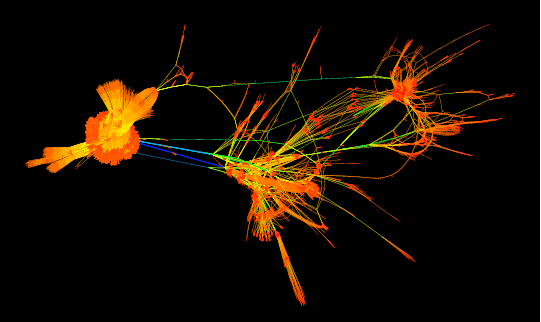
\includegraphics[width=.46\textwidth, height=4.3cm]{aor} }}%
    \qquad
  \subfloat[coarsened]{{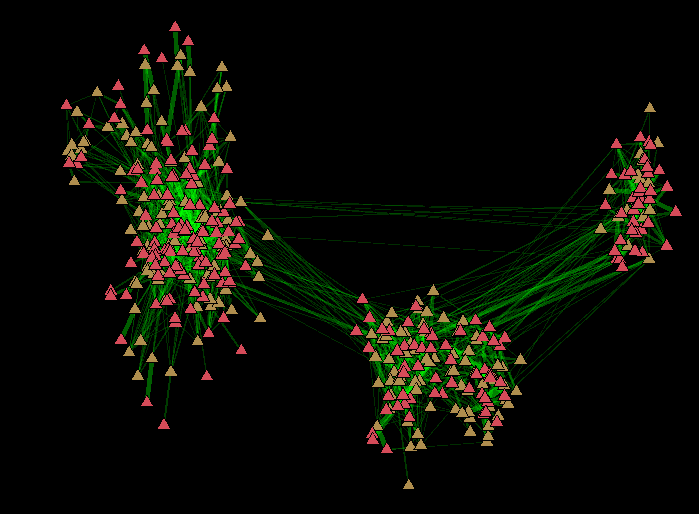
\includegraphics[width=.46\textwidth, height=4.3cm]{aml} }}%
    \caption{Graphical representations of a network with 24,211 nodes (8,788 proteins and 15,422 n-reactome iterations), and 41,087 links.
    In (a) the original network is mapped visually, and in (b) the network is represented using only 200 nodes (100 nodes in each layer).
    }%
    \label{aml0}%
\end{figure}

For this case study, we focused in the smallest of the three communities,
in order to visualize it separately,
observe its connectivity patterns,
and consequently the functional patterns
of the nodes that belong to this community.
Figures~\ref{aml1} (a), (b) and (c) depict the community in levels 2, 1 and 0 (original), respectively.
The final result is isolated in Figure~\ref{amlf},
were only the community is visualized, and only with uncoarsened nodes.
Therein, it is evident that a group of more connected nodes exists, they are in the center of the image.
The analist may wish, e.g., to target the genes among such nodes
in further steps of the investigation,
due to their central role in interacting with numerous proteins.
Another possibility is to examine the less connected nodes in an attempt
to understand their specific roles.

\begin{figure}[!h]\centering
    \subfloat[original]{{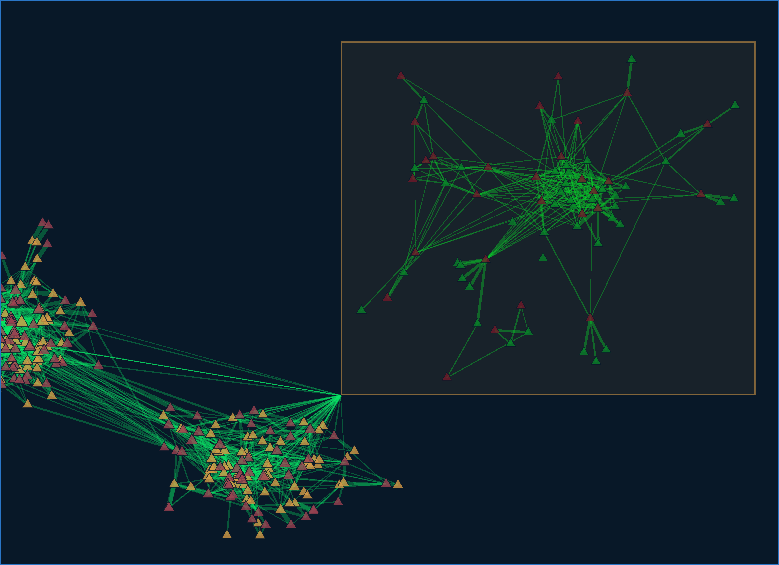
\includegraphics[width=.3\textwidth, height=3.3cm]{aml2} }}%
  \subfloat[coarsened]{{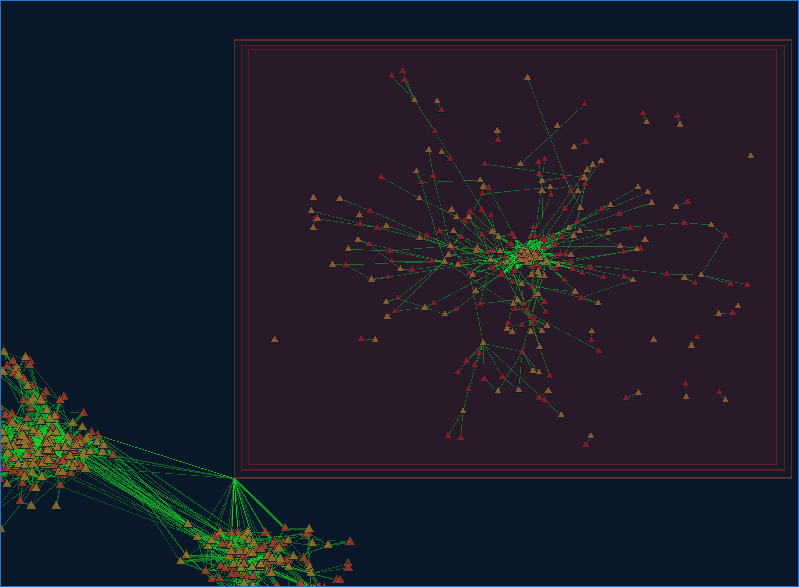
\includegraphics[width=.3\textwidth, height=3.3cm]{aml3} }}%
  \subfloat[coarsened]{{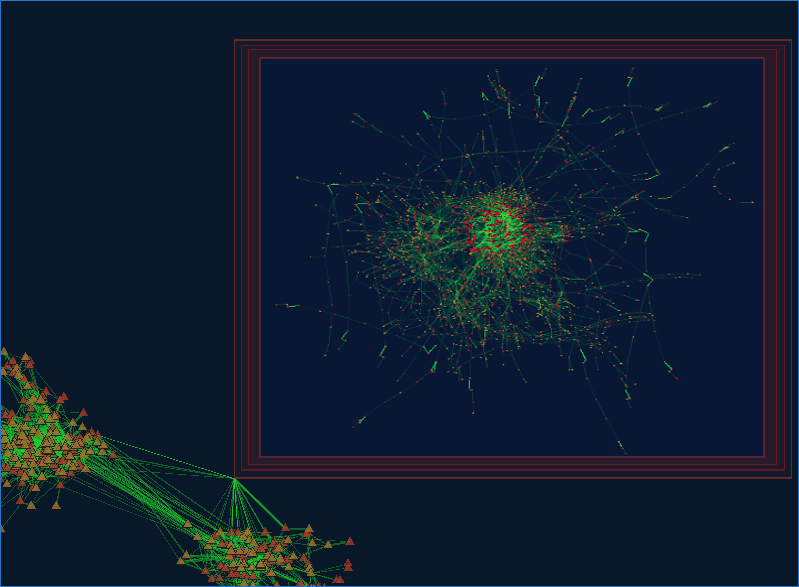
\includegraphics[width=.3\textwidth, height=3.3cm]{aml4_} }}%
    \caption{Progressive visualization of the smallest community if Figure~\ref{aml0}. In (a), the nodes are uncoarsened to level 2.
    In (b), the nodes are uncorsened to level 1.
    In (c), the noeds are uncoarsened to level 0, i.e. to the level of the original, uncoarsened, network.}%
    \label{aml1}%
\end{figure}

\begin{figure}\centering
 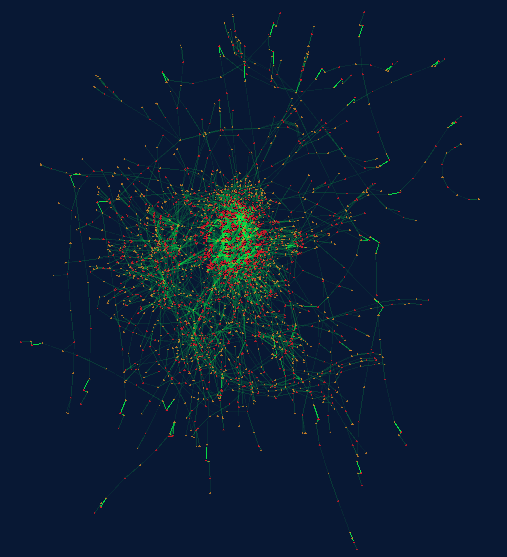
\includegraphics[width=0.7\textwidth,height=7cm]{aml5_}
  \caption{An isolated visualization of the community being analysed.
  The researcher reached this visualization by on-demand transformations of the initial visualization, i.e. from a respresentation with only 200 nodes of a network with 24,211 nodes.}\label{amlf}
\end{figure}

As exempified,
given the importance of the connectivity patterns,
such as group structure,
and given the effectiveness of the visualization assisted by multilevel strategies in bipartite networks,
the method may assist research related to gene/protein networks.
Thus, BiNetVis is potentially helpful in studying pathogenic variants,
groups of genes associated with metabolic deficiency,
or groups of proteins that can be targeted for therapeutic goals.

\FloatBarrier
\section*{Appendix C: The toolbar}
One special element that enables the interactive visualization of BiNetVis is the toolbar. It is contextualized in Figures~\ref{fpage0} and~\ref{secondPhase},
but in a scale which may not favor its inspection by the reader, specially in a printed version of this document.
Figure~\ref{toolbar} is dedicated to the toolbar and its usage is described in Section~\ref{use}.


\begin{figure}\centering
 
\includegraphics[width=\textwidth]{toolbar}
  \caption{The toolbar, contextualized in Figures~\ref{fpage0} and~\ref{secondPhase}, shown independently. The four groups of buttons are for transformations of: nodes, links, special/multilevel, and whole network. The usage is described in Section~\ref{use}.}\label{toolbar}
\end{figure}

\end{document}

